%\documentclass[10pt,xcolor={x11names}]{beamer}
\documentclass{falconbeamer}

%%%%%%%%%%%%%%%%%%%%%%%%%%%
%% Document informations %%
%%%%%%%%%%%%%%%%%%%%%%%%%%%

\renewcommand{\getdoctitle}{Reconnaissance efficace d’objets sous-marins}
\renewcommand{\getdocdate}{TIPE 2020}
%\newcommand{\getdocsubtitle}{Sous-titre du document}
\institute{
	\begin{center}
		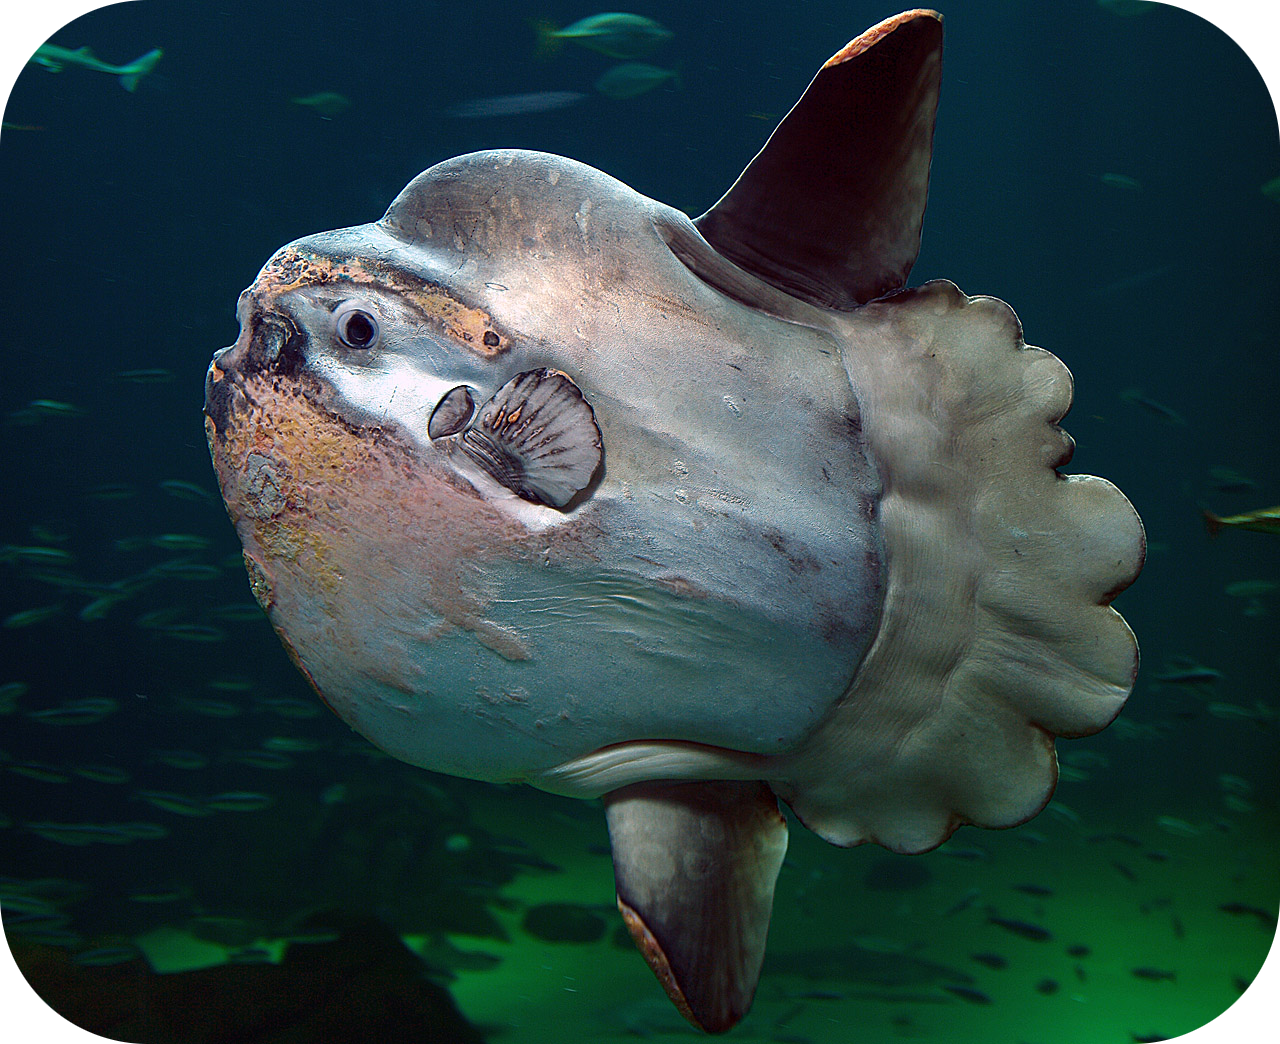
\includegraphics[height=.4\textheight]{molamola.png}
	\end{center}
}

%%%%%%%%%%%%%%%%%%%%%%
%% Document content %%
%%%%%%%%%%%%%%%%%%%%%%

\begin{document}

\maketitle

\begin{frame}{Le problème étudié}
	\bigskip
	\begin{columns}[T]
		\column{0.5\textwidth}
			\sectitle{Le problème}
			\begin{itemize}
				\item Reconnaissance d'espèces marines et d'objets sous l'eau
				\item En temps réel :
				\begin{itemize}
					\item Classification
					\item Apprentissage de nouvelles données
					\item Detection d'objets inconnus
				\end{itemize}
			\end{itemize}
		
		\column{0.5\textwidth}
			\sectitle{Les aspects difficiles}
			\begin{itemize}
				\item Complexité des fonds marins
				\item Diversité des espèces
				\item Peu de données pour certaines classes
			\end{itemize}
	\end{columns}
	\begin{columns}
		\column{0.7\textwidth}
			\begin{center}
			\sectitle{Utilité pratique}
			\end{center}
			\begin{itemize}
				\item Sous-marins autonomes
				\item Etudes non-destructive des populations
				\item Faibles coûts
			\end{itemize}
	\end{columns}
\end{frame}

\begin{frame}{Données utilisée}
	\begin{center}
		\begin{tabular}{ |m{14em}|m{14em}| }
			\hline
			\textbf{Fish4Knowledge species (F4K)} & \textbf{Images depuis Google (G)}  \\
			\hline\smallskip
			23 espèces & 150 espèces \\
			\smallskip
			12 122 images à 25 par espèce & 10 images par espèce \\
			Autour de $100\times100$ pixels & $128\times128$ pixels \\
			\hline
		\end{tabular} \\
		\bigskip
		\sectitle{Sous-sets de données}
		Origine des données et nombre d'images par espèce : \\
		\medskip
		\begin{tabular}{ |m{6.5em}|m{6.5em}|m{6.5em}|m{6.5em}| }
			\hline
			\textbf{3 espèces} & \textbf{6 espèces} &  \textbf{23 espèces} &  \textbf{173 espèces}\\
			\hline\smallskip
			F4K & F4K & F4K & F4K + G \\
			3200 à 4000 & 148 à 4000 & 25 à 4000 & 10 \\
			\hline
		\end{tabular}
	\end{center}
\end{frame}

\begin{frame}{Implémentation}
	\begin{columns}
		\column{0.5\textwidth}
		% python + DML + theano + local CPU
		\begin{center}
			\sectitle{Modèles légers}
			\medskip
			
\includegraphics[height=1.5em]{python.png}\\\smallskip
			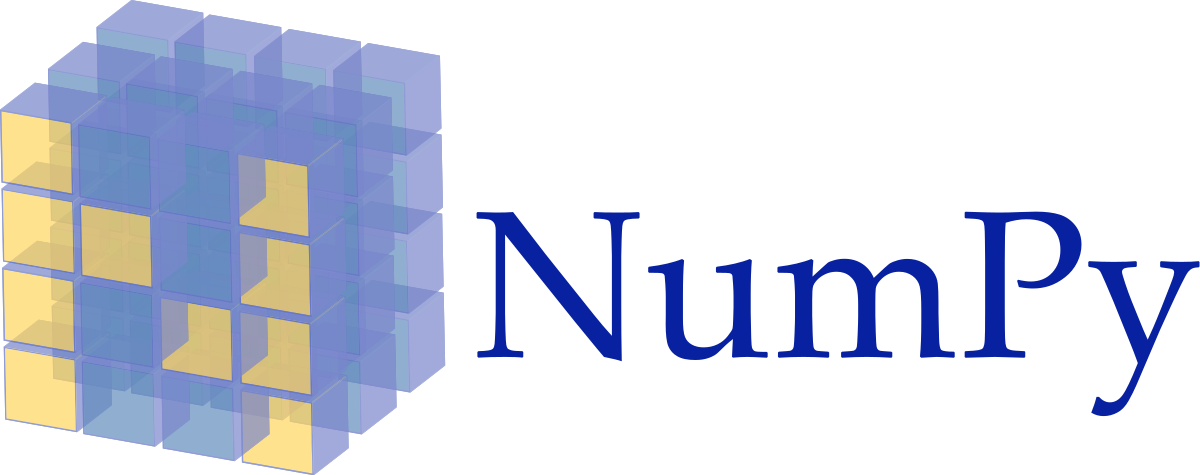
\includegraphics[height=1.5em]{numpy.png}\\\smallskip
			\textbf{\Large DML} \\\smallskip
			
\includegraphics[height=1.5em]{theano.png} \\\smallskip
			CPU local
		\end{center}
		
		\column{0.5\textwidth}
		% python + tf.Keras + tensorflow + GPU
		\begin{center}
			\sectitle{Modèles lourds}
			\medskip
			
\includegraphics[height=1.5em]{python.png}\\\smallskip
			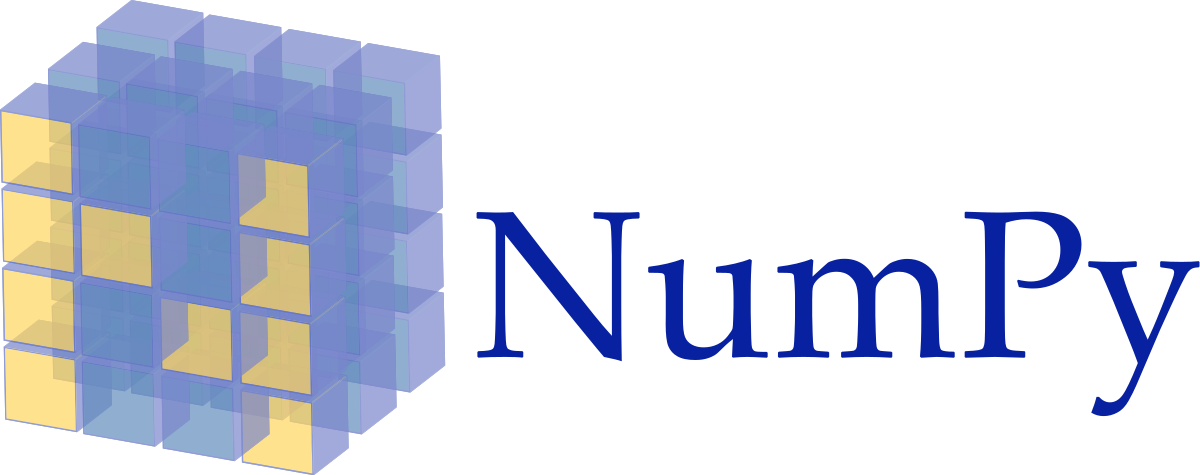
\includegraphics[height=1.5em]{numpy.png}\\\smallskip
			
\includegraphics[height=1.5em]{keras.png} \\\smallskip
			
\includegraphics[height=1.5em]{tensorflow.png} \\\smallskip
			\raisebox{-.25\height}{
\includegraphics[height=1.5em]{colab.png}} (GPU)
		\end{center}
	\end{columns}
	\begin{center}
		\sectitle{Classification rapide avec K plus proche voisins}
		\medskip
		
\includegraphics[height=2.5em]{cpp.png}
	\end{center}
\end{frame}

\section{Premières méthodes de classification}

\begin{frame}{Distances euclidiennes}
	\begin{columns}[T]
		\column{0.5\textwidth}
		\sectitle{K plus proches voisins (KNN)}
		\begin{itemize}
			\item Dimension $30 000$
			\item Dépend de la position de l'objet sur l'image
		\end{itemize}
		
		\column{0.5\textwidth}
		\sectitle{Densité de couleurs}
		\begin{itemize}
			\item Dimension $3$
			\item Indépendant de la position de l'objet
		\end{itemize}
	\end{columns}
	
	\begin{center}
		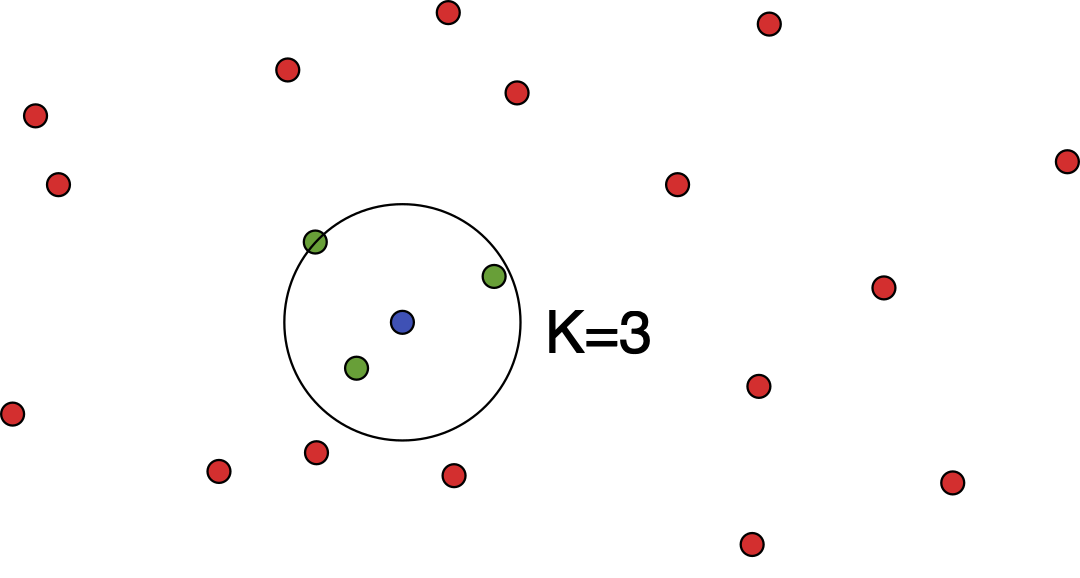
\includegraphics[width=.4\textwidth]{KNN.png}
		
		\begin{tabular}{ |m{6.5em}|m{6.5em}|m{6.5em}|m{6.5em}| }
			\hline
			& \textbf{3 espèces} & \textbf{6 espèces} &  \textbf{23 espèces} \\
			\hline\smallskip
			\textbf{KNN} & $91.6\%$ & $87.87\%$ & $38.84\%$ \\\smallskip
			\textbf{Densité} & $67.50\%$ & $39.73\%$ & $21.4\%$ \\\smallskip
			\textbf{Aléatoire} & $33.33\%$ & $16.67\%$ & $4.32\%$ \\
			\hline
		\end{tabular}
	\end{center}
	
	%\begin{theorem};
	%	Hey ! f(x)=42
	%\end{theorem}
\end{frame}

\begin{frame}{Construction d'un réseau de neurones (ANN)}
	\begin{block}{Ce qu'est réellement un ANN}
		Un réseau de neurones est une manière de représenter certaines fonctions non-linéaires
	\end{block}

	\begin{columns}
		\column{0.25\textwidth}
		\begin{flushright}
			\resizebox{4.5em}{!}{$\begin{pmatrix} a_{1}\\ a_{2}\\ \vdots \\ a_{n} \end{pmatrix}$}
		\end{flushright}
		\column{0.5\textwidth}
		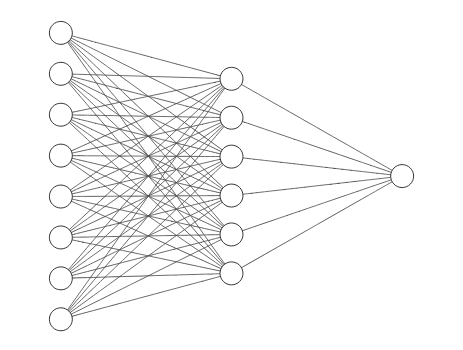
\includegraphics[width=\textwidth]{nnet.png}
		\column{0.25\textwidth}
		\resizebox{4em}{!}{$\begin{pmatrix} y_{1}\\ y_{2}\\ \vdots \\ y_{n} \end{pmatrix}$}
	\end{columns}
\end{frame}

\begin{frame}{Fonctionnement d'un neurone}
	\begin{center}
		\tikzimg{how_neuron_works}
	\end{center}
	\begin{columns}
		\column{0.5\textwidth}
		$$
			z=b+\sum_{i=1}^na_i\times b_i
		$$
		\medskip
		$$
		y=\sigma(z)
		$$
		
		
		\column{0.5\textwidth}
		\arrayrulecolor{lightgray}
		\begin{tabular}{ |c|c| }
			\hline
			{\footnotesize Sigmoïde}  & {\footnotesize Tanh} \\
			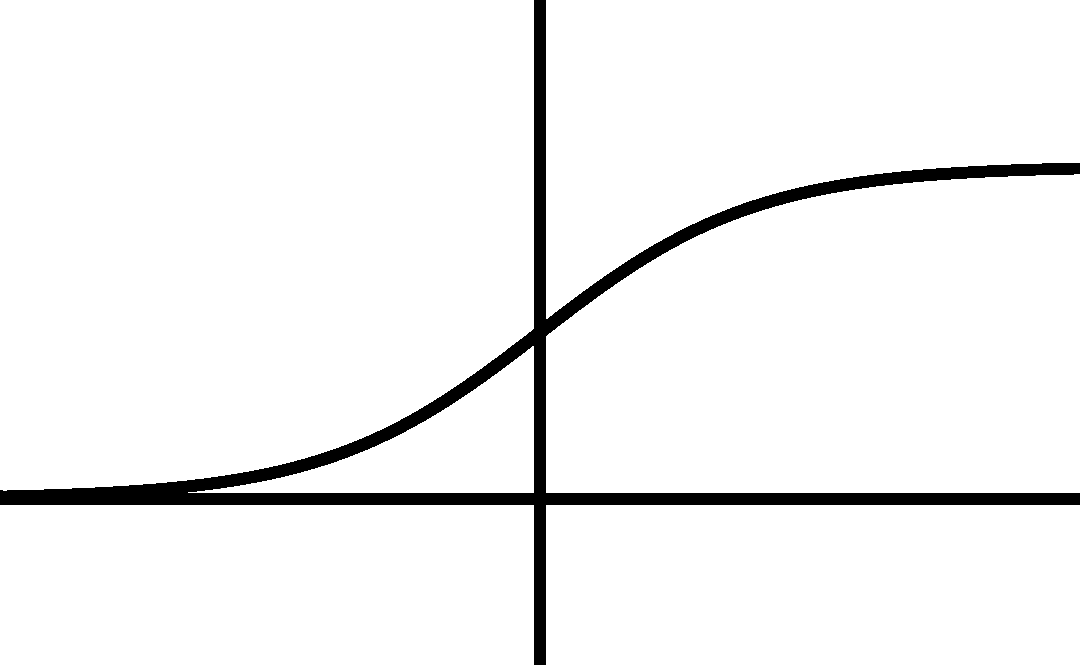
\includegraphics[width=5em]{sigmoid.png}& 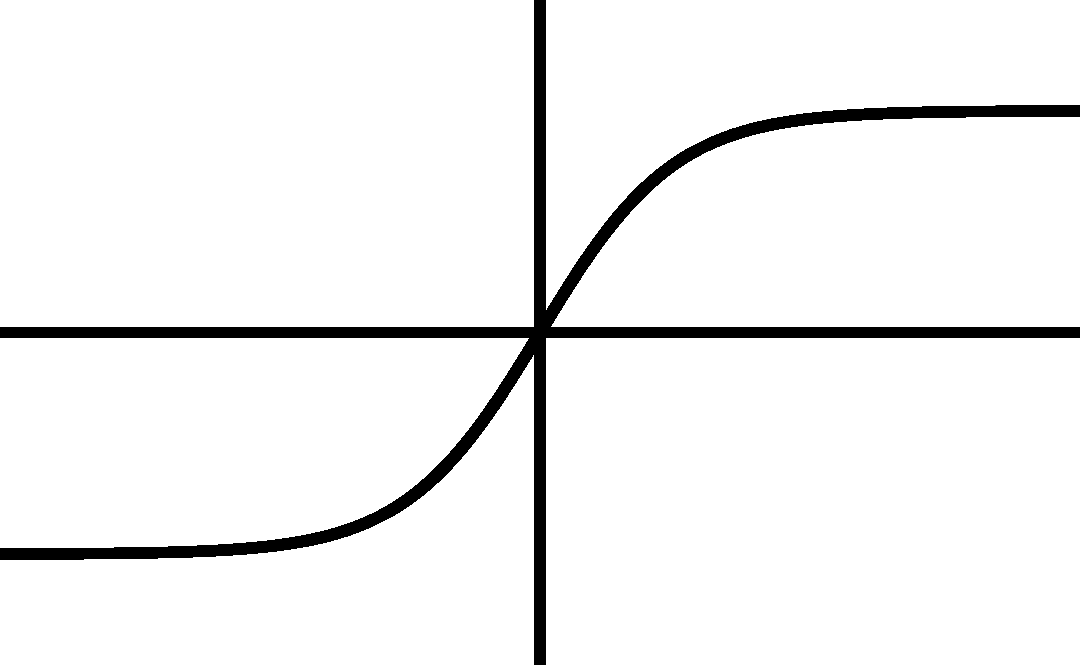
\includegraphics[width=5em]{tanh.png} \\
			$y=\frac{1}{1+e^{-z}}$ & $y=tanh(z)$ \\
			\hline
			{\footnotesize ReLU}  & {\footnotesize Weak ReLU} \\
			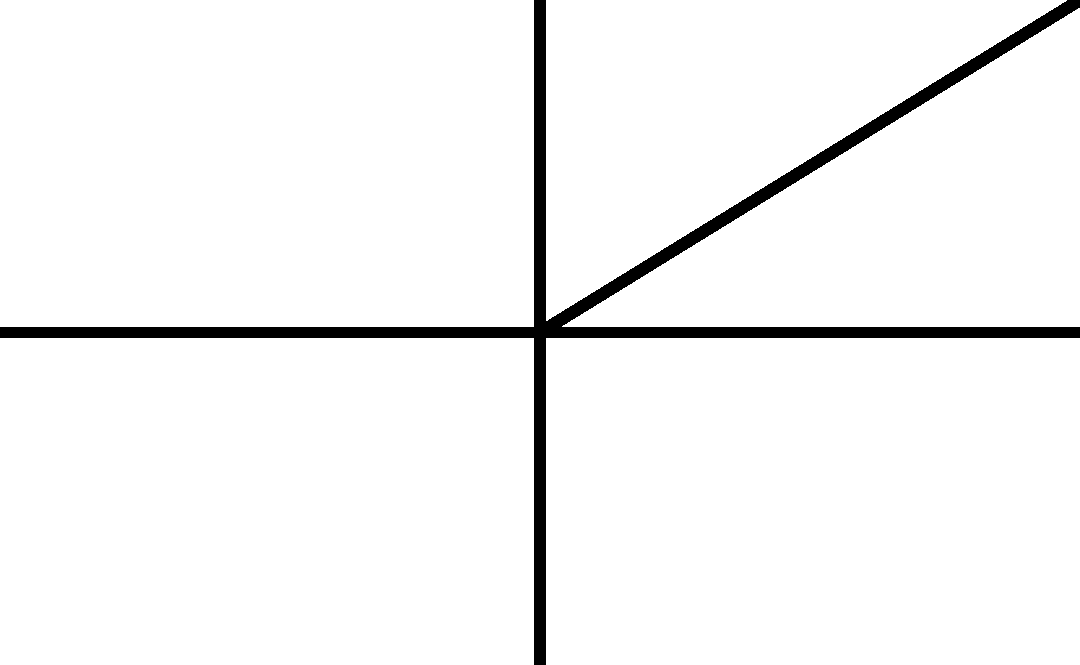
\includegraphics[width=5em]{relu.png}& 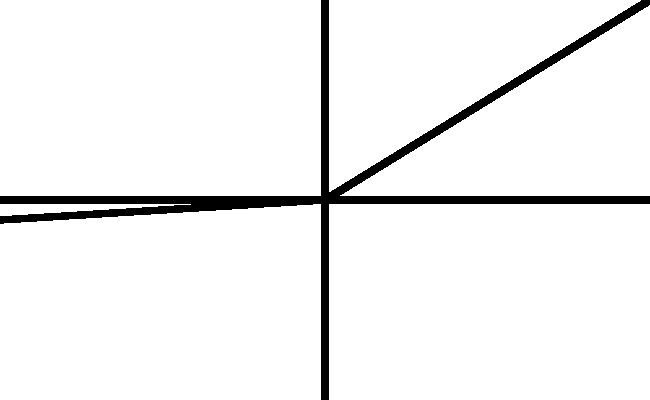
\includegraphics[width=5em]{weakrelu.png} \\
			$y=max(0,z)$ & $y=max(\epsilon\times z, z)$ \\
			\hline
		\end{tabular}
		\arrayrulecolor{black}
	\end{columns}
\end{frame}

\begin{frame}{Couche dense de neurones}
	\begin{columns}
		\column{0.3\textwidth}
		\begin{flushright}
			\resizebox{2em}{!}{$A^l$}
		\end{flushright}
		\column{0.4\textwidth}
		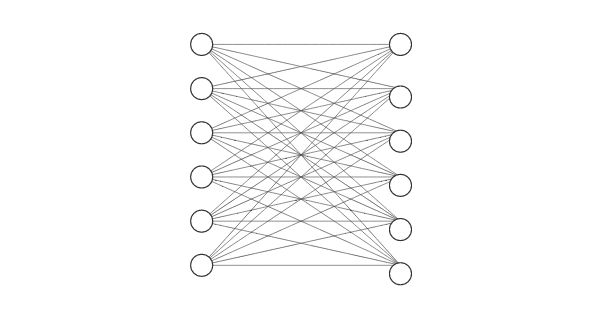
\includegraphics[width=\textwidth]{couche.png}
		\column{0.3\textwidth}
		\resizebox{2em}{!}{$Y^l$}
	\end{columns}
	\begin{columns}
		\column{0.3\textwidth}
		$$
		Z^l=W^l\times A^l+B^l
		$$
		$$
		Y^l=\sigma(Z^l)
		$$
		
		\column{0.3\textwidth}
		$$
			W=\begin{pmatrix} 
			w_{1,1} & \cdots &w_{1,n} \\
			w_{2,1} & \cdots &w_{2,n} \\
			\vdots & \ddots & \vdots \\
			w_{p,1} & \cdots &w_{p,n}
			\end{pmatrix}
		$$
		
		\column{0.3\textwidth}
		$$
			A=\begin{pmatrix}
			a_1 \\
			a_2 \\
			\vdots \\
			a_n
			\end{pmatrix}\ \ 
			B=\begin{pmatrix}
			b_1 \\
			b_2 \\
			\vdots \\
			b_p
			\end{pmatrix}
		$$
	\end{columns}
	\begin{center}
		$W^l$ et $B^l$ sont appris.
	\end{center}
	
\end{frame}

\begin{frame}{Entraînement}
	\begin{columns}[T]
		\column{0.5\textwidth}
		\sectitle{Fonction de coût $L_2$}
		$$
		C=\frac{1}{m}\sum_{i=1}^m (\hat{y}_i-y_i)^2
		$$
		Avec :
		\begin{itemize}
			\item $m$ : nombre d'images
			\item $\hat{y}$ : sortie attendue
		\end{itemize}
		\column{0.5\textwidth}
		\sectitle{Descente de gradient}
		$$
		W' = W - \lambda \frac{\partial C}{\partial W}
		$$
		$$
		B' = B - \lambda \frac{\partial C}{\partial B}
		$$
		{\centering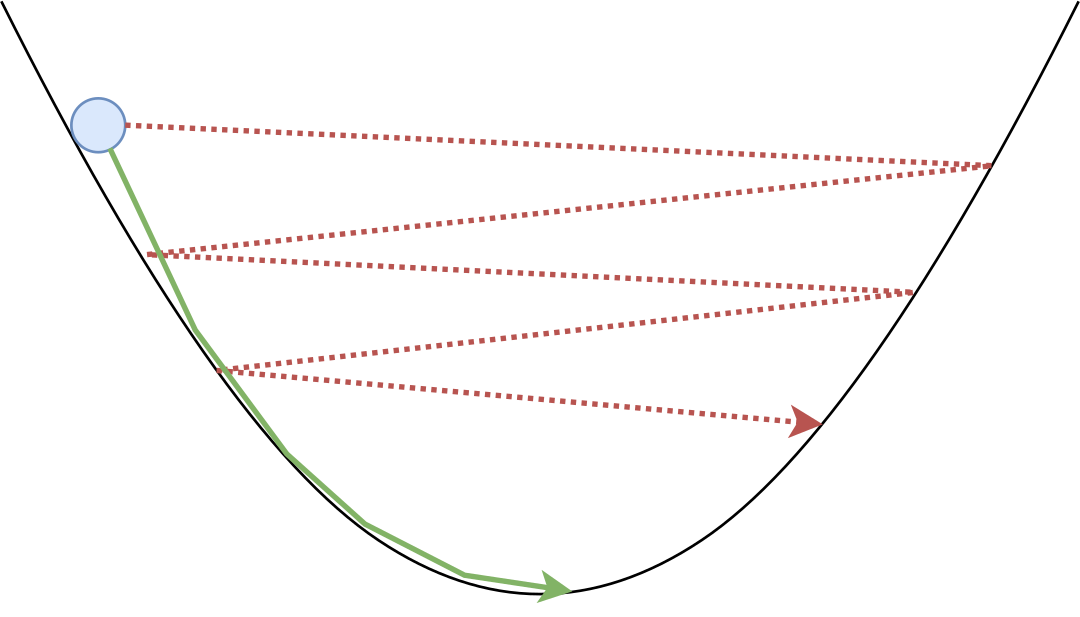
\includegraphics[width=\textwidth]{gradient.png}}
	\end{columns}
\end{frame}

\begin{frame}{Résultats intermédiaires 1}
	\begin{tabular}{ |m{10em}|m{5.5em}|m{5.5em}|m{5.5em}| }
		\hline
		Modèle & \textbf{3 espèces} & \textbf{6 espèces} &  \textbf{23 espèces} \\
		\hline
		\textbf{Aléatoire} & $33.33\%$ & $16.67\%$ & $4.32\%$ \\
		\textbf{KNN} & $91.6\%$ & $87.87\%$ & $38.84\%$ \\
		\textbf{ANN dense} & $96.83\%$ & $95.20\%$ & $83.58\%$ \\
		\hline
	\end{tabular}
	\begin{center}
	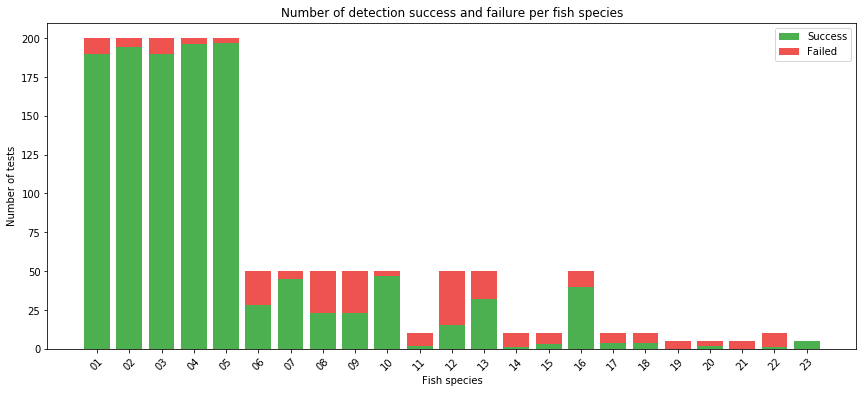
\includegraphics[width=\linewidth]{dense1_results.png}
	\end{center}
\end{frame}

\begin{frame}{Améliorer l'entrainement}
	\begin{columns}[T]
		\column{0.5\textwidth}
		\sectitle{Ajouter un moment au gradient [FAUX !!!]}
		$$
		M_W=M_W - \lambda \frac{\partial C}{\partial W}
		$$
		$$
		W=W + M_W
		$$
		{\centering 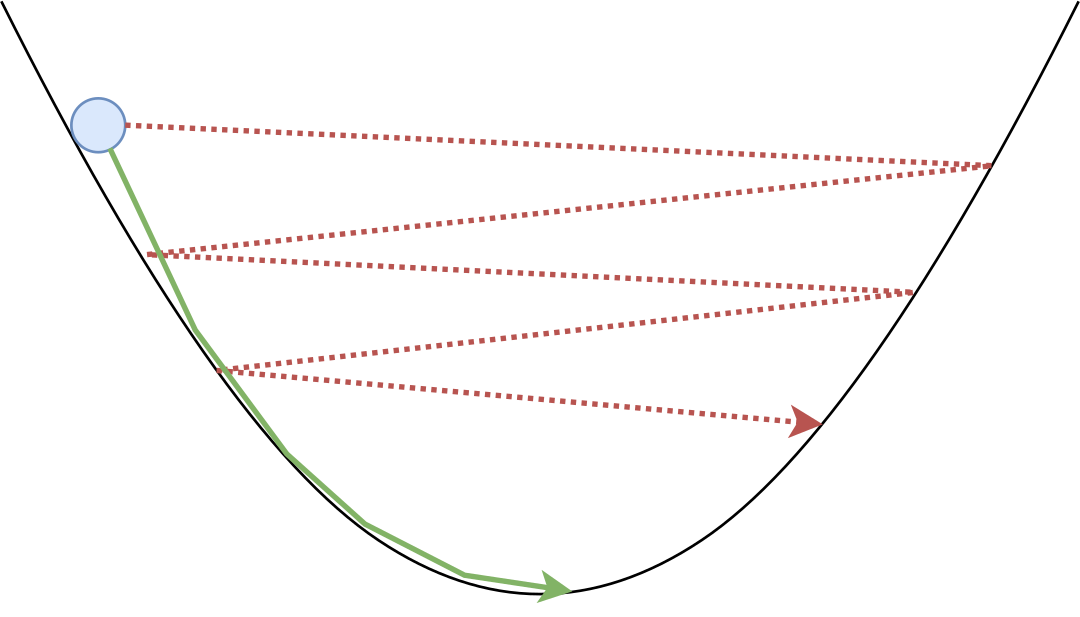
\includegraphics[width=0.9\textwidth]{gradient.png}}
		
		\column{0.5\textwidth}
		\sectitle{Couche softmax}
		Distribution de probabilité
		$$
		y^L_j=\frac{e^{z_j^L}}{\sum_i e^{z_i^L}}
		$$
		\medskip
		\textbf{Fonction de coût log-likelihood}
		$$
		C=-\log(y^L_{i_0})
		$$
		On a $\hat{y}$ de la forme $[0,\dots,0,1,0,\dots,0]$, et $\hat{y}_{i_0}=1$
		
	\end{columns}
\end{frame}

\begin{frame}{Normalisation}
	\begin{columns}[T]
		\column{0.45\textwidth}
		\sectitle{Entrées}
		$$
		\mu=\frac{1}{n}\sum_{i=1}^nX^{(i)}
		$$
		$$
		\sigma=\sqrt{\frac{1}{n}\sum_{i=1}^n(X^{(i)}-\mu)^2}
		$$
		
		Avec le carré élément par élément (au sens du produit de Hadamard).
		
		$$
		X^\prime=\frac{X-\mu}{\sigma}
		$$
		
		\column{0.55\textwidth}
		\sectitle{Activations}
		
		\begin{itemize}
			\item $\mu$ et $\sigma$ calculés par batchs
			\item $\alpha$ et $\beta$ paramètres appris
			\item $\gamma\in]0;1[$ fixe
		\end{itemize}
	
		{\centering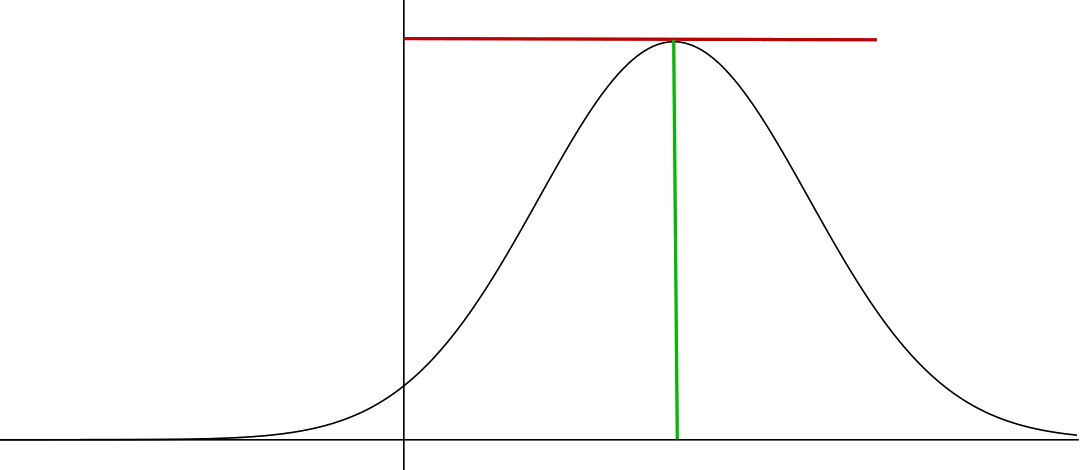
\includegraphics[width=0.8\textwidth]{gaussian.png}}
		
		
		$$
		\hat{\mu}=\gamma\hat{\mu}+(1-\gamma)\hat{\mu}
		\ \ \ \ \ \ \text{et} \ \ \ \ \ \ \hat{\sigma}=\gamma\hat{\sigma}+(1-\gamma)\hat{\sigma}
		$$
		
		$$
		a_{\text{norm}}=\alpha\frac{a-\hat{\mu}}{\hat{\sigma}}+\beta
		$$
	\end{columns}
\end{frame}

\begin{frame}{Résultats intermédiaires 2}
	\begin{tabular}{ |m{10em}|m{5.5em}|m{5.5em}|m{5.5em}| }
		\hline
		Modèle & \textbf{3 espèces} & \textbf{6 espèces} &  \textbf{23 espèces} \\
		\hline
		\textbf{Aléatoire} & $33.33\%$ & $16.67\%$ & $4.32\%$ \\
		\textbf{KNN} & $91.6\%$ & $87.87\%$ & $38.84\%$ \\
		\textbf{ANN dense} & $96.83\%$ & $95.20\%$ & $83.58\%$ \\
		\textbf{ANN dense amélioré} & $99.33\%$ & $95.60\%$ & $91.35\%$ \\
		\hline
	\end{tabular}
	\begin{center}
		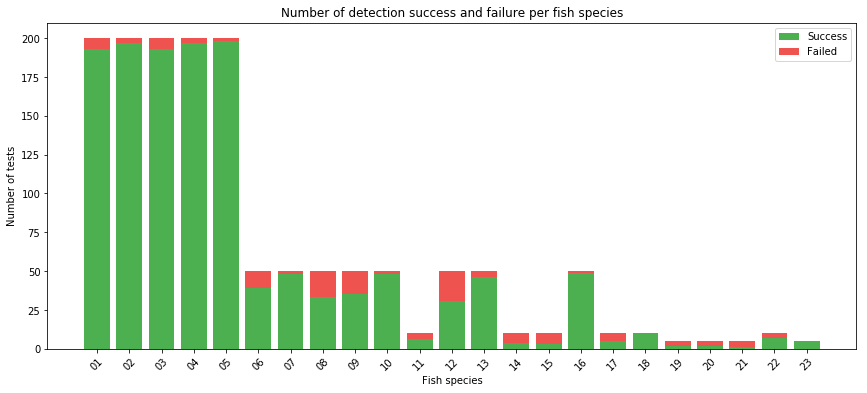
\includegraphics[width=\linewidth]{dense2_results.png}
	\end{center}
	
\end{frame}

\begin{frame}{Convolutions}
	Nouveau type de couche, utilisé pour créer un ConvNet. La matrice des filtres d'une couche sera une matrice 4D.
	\begin{center}
		\includegraphics[width=0.8\textwidth]{conv_net1.png}\\
		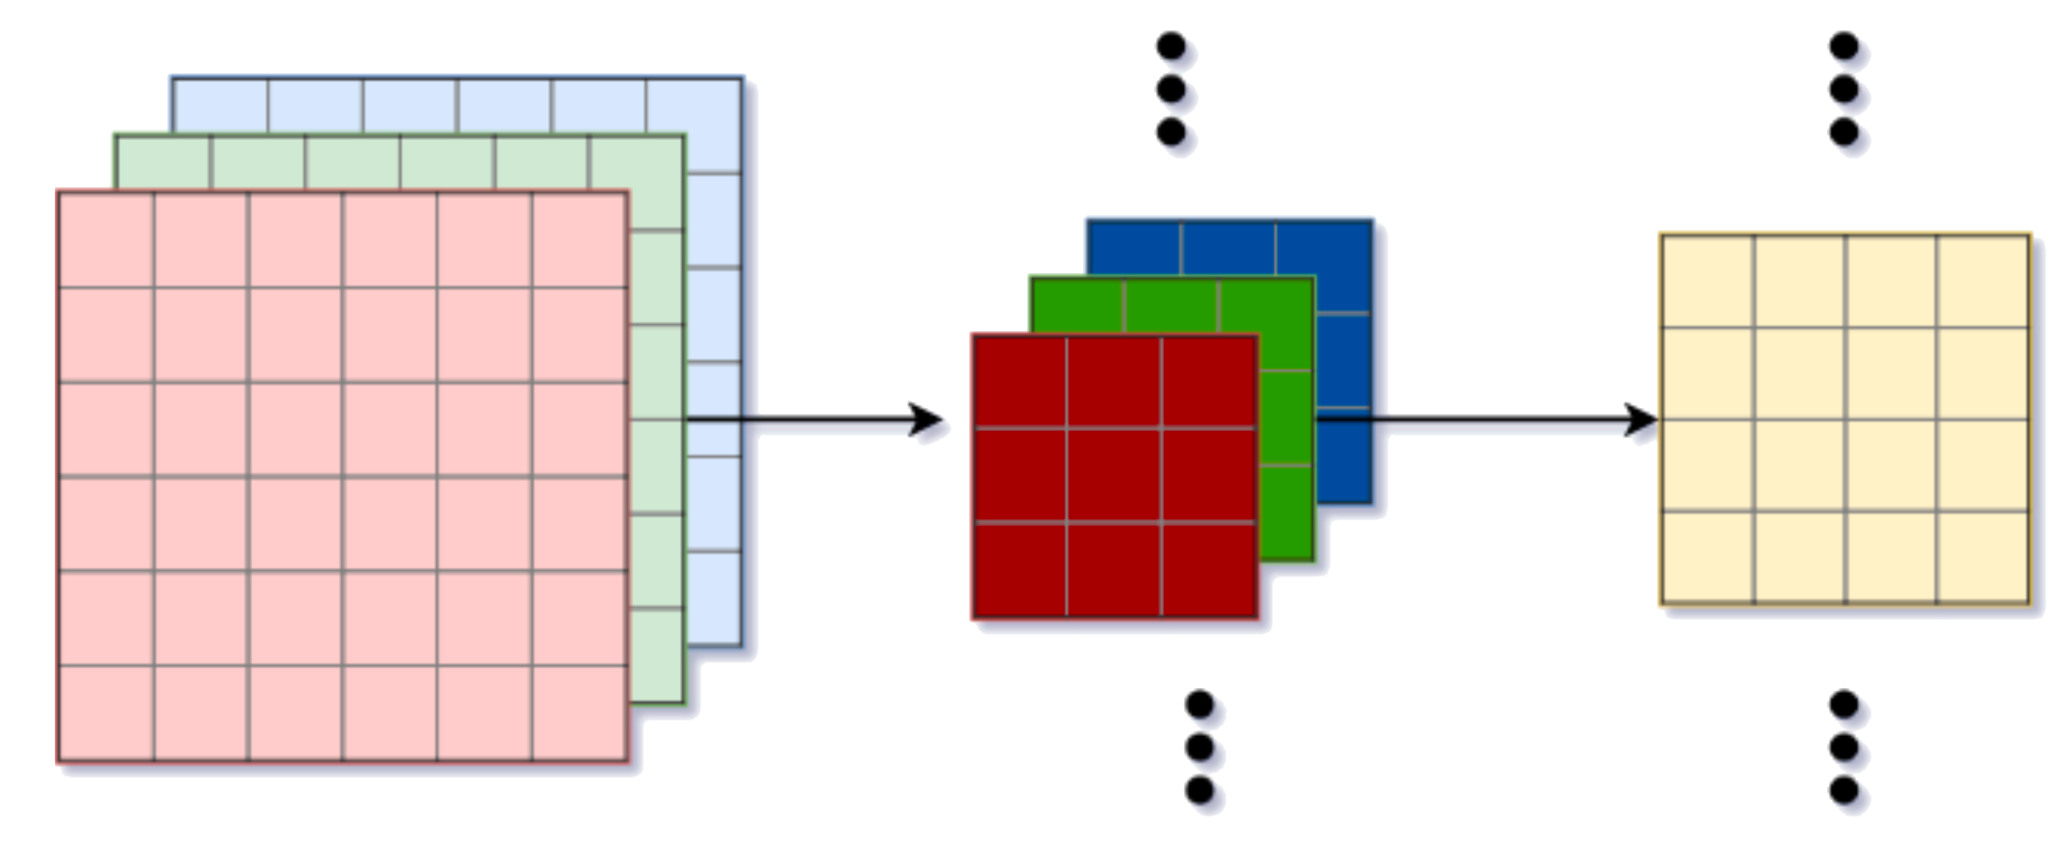
\includegraphics[width=0.7\textwidth]{conv_channels.png}
	\end{center}
\end{frame}

\begin{frame}{Pooling}
	Couche de max-pooling, suit une couche de convolution.
	\begin{center}
		\includegraphics[width=\textwidth]{maxpool.png}
	\end{center}
	Réduit la dimension spatiale et sélectionne l'information.
\end{frame}



\begin{frame}{Résultats intermédiaires 3}
	\begin{tabular}{ |m{10em}|m{5.5em}|m{5.5em}|m{5.5em}| }
		\hline
		Modèle & \textbf{3 espèces} & \textbf{6 espèces} &  \textbf{23 espèces} \\
		\hline
		\textbf{Aléatoire} & $33.33\%$ & $16.67\%$ & $4.32\%$ \\
		\textbf{KNN} & $91.6\%$ & $87.87\%$ & $38.84\%$ \\
		\textbf{ANN dense} & $96.83\%$ & $95.20\%$ & $83.58\%$ \\
		\textbf{ANN dense amélioré} & $99.33\%$ & $95.60\%$ & $91.35\%$ \\
		\textbf{ConvNet} & $99.50\%$ & $97.73\%$ & $96.96\%$ \\
		\hline
	\end{tabular}
	\begin{center}
		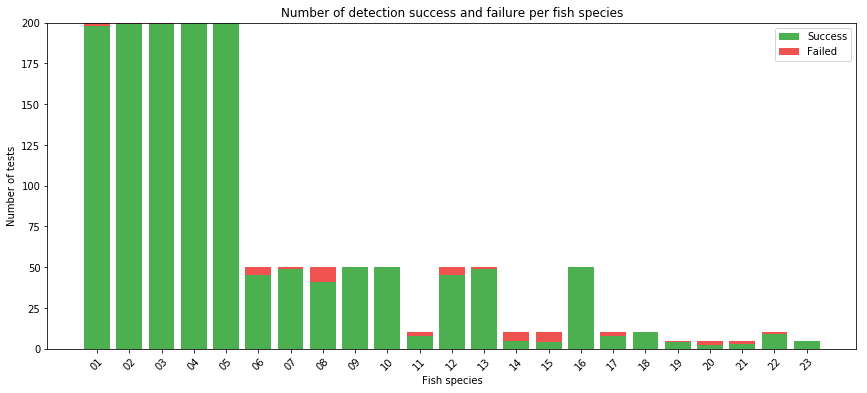
\includegraphics[width=\linewidth]{conv2_results.png}
	\end{center}
	
\end{frame}

\begin{frame}{Architectures}
	\begin{center}
		\sectitle{ANN dense}
		Paramètres : $102,787,095$\\
		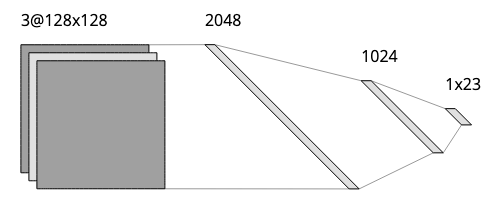
\includegraphics[width=0.66\textwidth]{dense_arch.png}
		\smallskip
		\newline
		\sectitle{ConvNet}
		Paramètres : $7,801,117$\\
		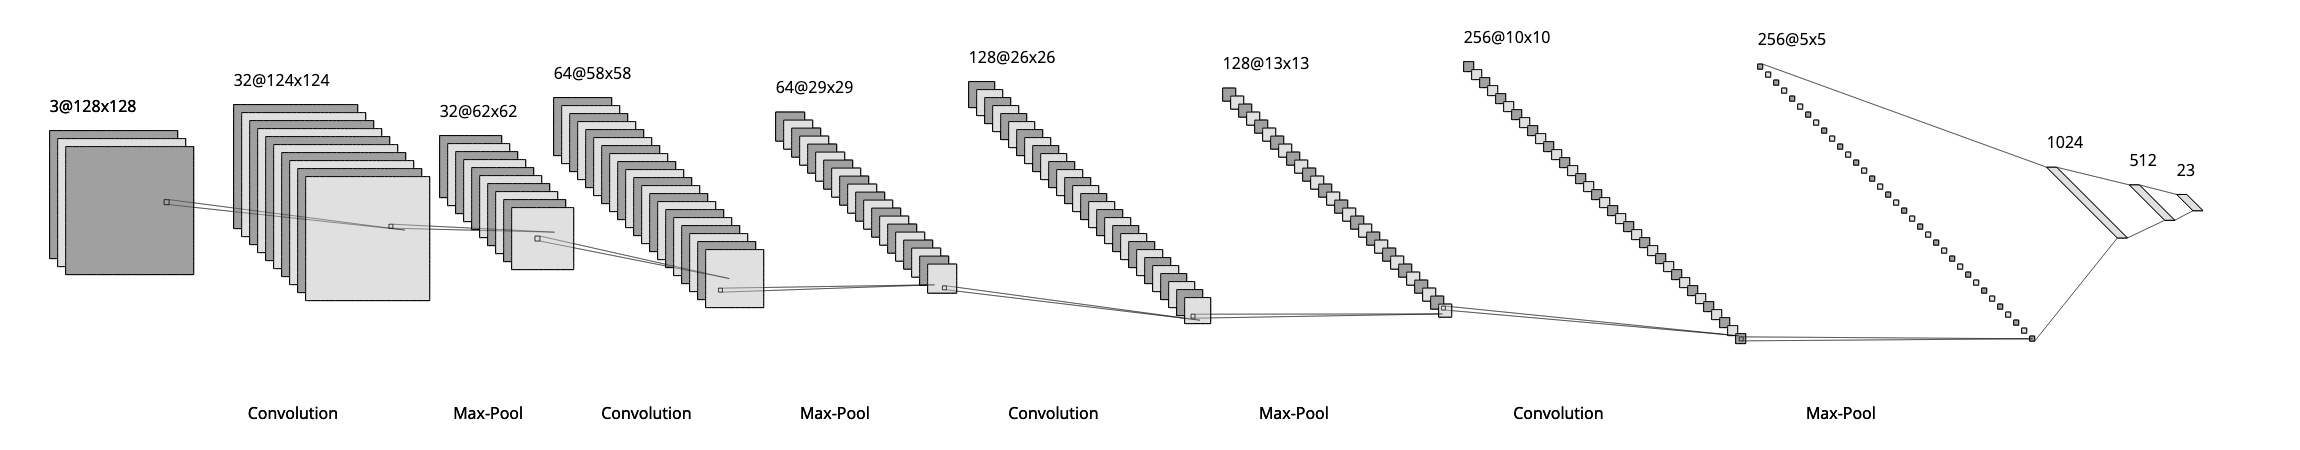
\includegraphics[width=1.1\textwidth]{conv2_arch.png}
	\end{center}
\end{frame}

\begin{frame}{Complexités}
	\begin{itemize}
		\item Pour une couche dense, $n$ et $m$ sont les tailles d'entrée et sortie
		\item Pour une couche de convolution :
		\begin{itemize}
			\item $n\times n\times m$ est la taille de l'entrée
			\item $k$ est la taille du filtre
			\item $l$ est le nombre de canaux de sortie
		\end{itemize}
	\end{itemize}
	\begin{center}
	\begin{tabular}{|c|c|}
		\hline
		\textbf{Opéation} & \textbf{Complexité} \\
		\hline
		Couche dense & $O(n\times m)$ \\
		\hline
		Convolution & $O(lmk^2n^2)$\\
		\hline
		Autres & $O(n)$\\
		\hline
	\end{tabular}
	\end{center}
\end{frame}

\begin{frame}{Limites}
	\begin{center}
		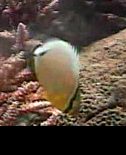
\includegraphics[width=4em]{fishes/5.png}
		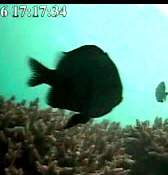
\includegraphics[width=4em]{fishes/1.png}
		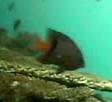
\includegraphics[width=4em]{fishes/2.png}
		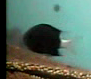
\includegraphics[width=4em]{fishes/3.png}
		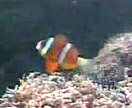
\includegraphics[width=4em]{fishes/4.png}
		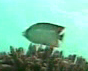
\includegraphics[width=4em]{fishes/6.png}
		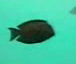
\includegraphics[width=4em]{fishes/8.png}
	\end{center}

	\begin{columns}
		\column{0.5\textwidth}
		\begin{itemize}
			\item Nombre de classes
			\item Temps d'entrainement :
			\begin{itemize}
				\item Ajout de données
				\item Ajout de classes
			\end{itemize}
		\end{itemize}
	\end{columns}

	\begin{center}
		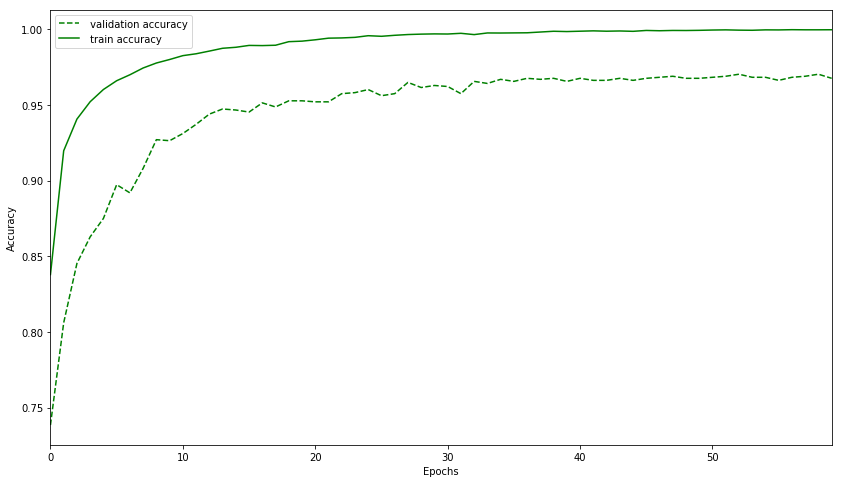
\includegraphics[width=12em]{train_3_acc.png}
		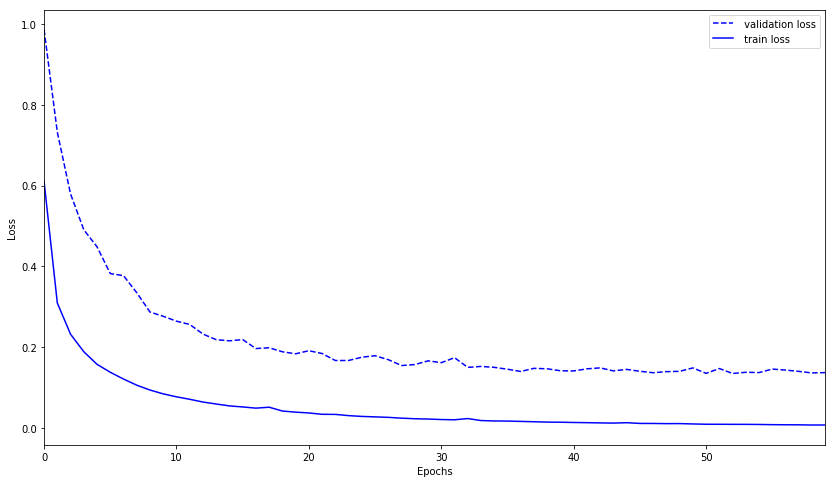
\includegraphics[width=12em]{train_3_loss.png}
	\end{center}
\end{frame}

\section{Transformation de l'image}

\begin{frame}{Ce que l'on cherche}
	\tikzimg{what_we_search}
\end{frame}

\begin{frame}{Réseau siamois}
	\begin{center}
		\tikzimg{siamese_schema}
	\end{center}
\end{frame}

\begin{frame}{Fonction de coût avec triplets}
	\begin{center}
		\tikzimg{triplet_cost}
	\end{center}
	On fixe la marge $m > 0$.
	$$
		C=max(0, d(a_a, a_p)-d(a_a, a_n))
	$$
\end{frame}

\begin{frame}{Sélectionner les triplets}
	
	\begin{center}
		\tikzimg{triplets}
	\end{center}
	
	\begin{block}{Algorithme rapide}
		- Un représentant par classe\\
		- Distance entre les représentants\\
		- Finalement, les 10 plus éloignés par image
	\end{block}

\end{frame}

\begin{frame}{Transfert d'apprentissage}
	\begin{center}
		\tikzimg{transfer_learning}
		\medskip
		\begin{columns}
			\column{0.5\textwidth}
			\sectitle{ConvNet}
			\begin{itemize}
				\item Entrainé sur F4K
				\item Spécialisé
				\item Ré-entrainé
			\end{itemize}
		
			\column{0.5\textwidth}
			\sectitle{MobileNet V2}
			\begin{itemize}
				\item Entrainé sur ImageNet
				\item Généraliste
				\item Utilisé tel quel
			\end{itemize}
		\end{columns}
		
	\end{center}
\end{frame}

\begin{frame}{Résultats}
	\begin{tabular}{ |m{10em}|m{8em}|m{8em}| }
		\hline
		Modèle & \textbf{173 espèces (entrainement)} & \textbf{23 espèces (test)} \\
		\hline
		\textbf{Aléatoire} & $0.58\%$ & $4.32\%$ \\
		\textbf{KNN} & $8.76\%$ & $38.8\%$ \\
		%\textbf{ConvNet} & - & $83.58\%$ \\
		\textbf{MobileNet + Siamois} & $26\%$ & $67\%$ \\
		\textbf{ConvNet + Siamois} & $91.85\%$ & $61.29\%$ \\
		\hline
	\end{tabular}
	\begin{center}
		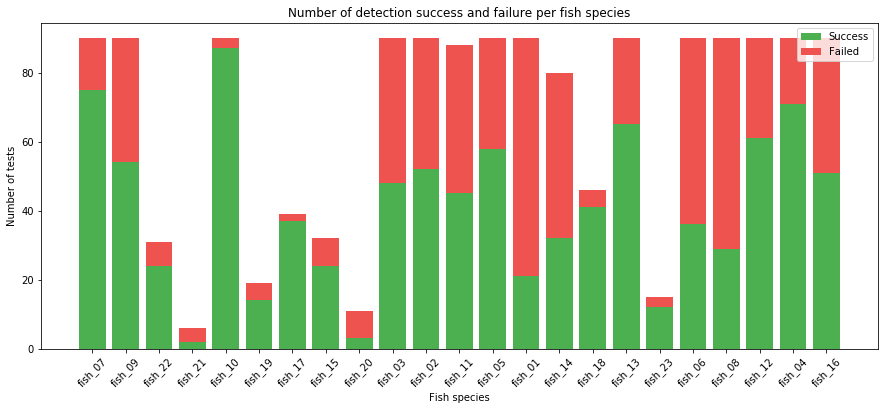
\includegraphics[width=\linewidth]{tl1_23out.png}
	\end{center}
\end{frame}

\begin{frame}{Statistiques sur l'entrainement}
	\begin{center}
		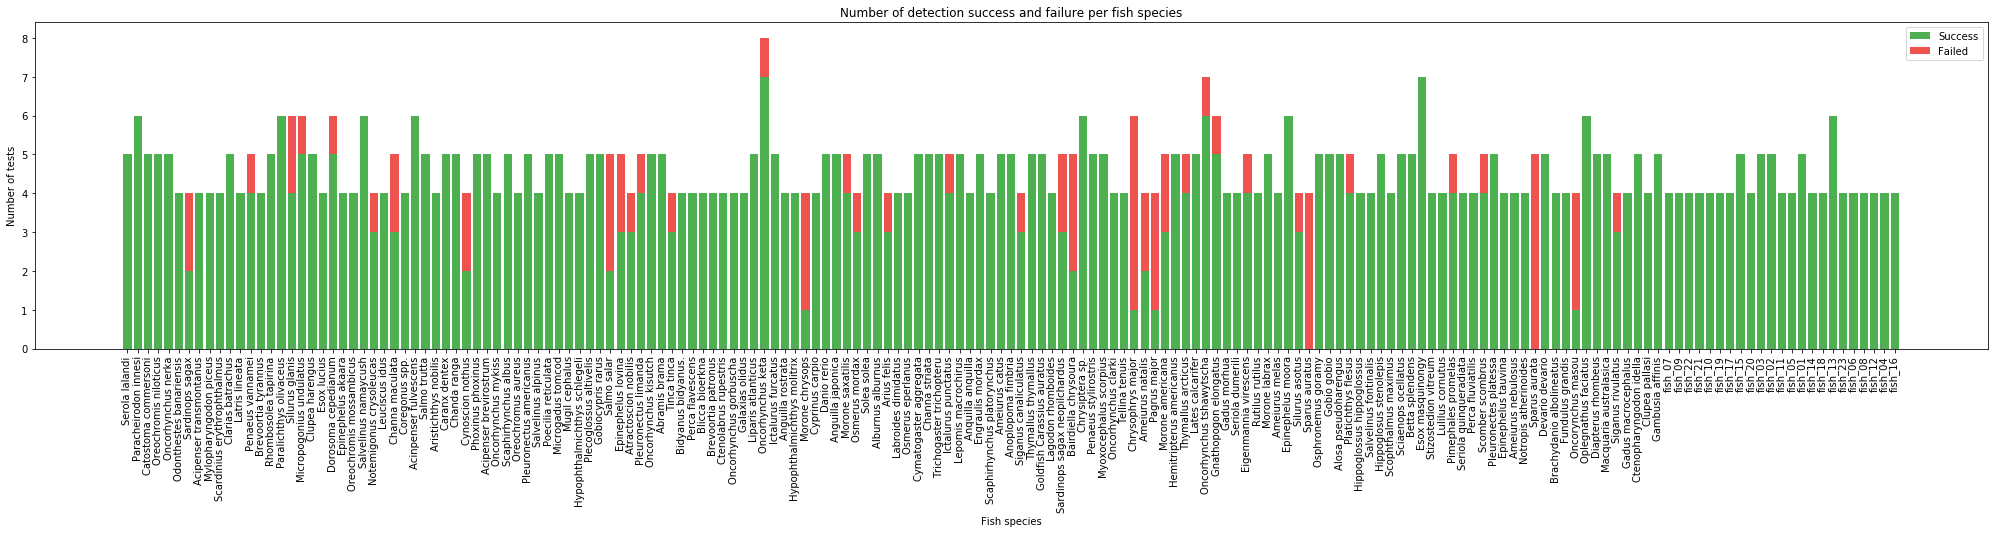
\includegraphics[width=30em,natwidth=1998,natheight=533]{stats1/tl1.2_150.png} \\
		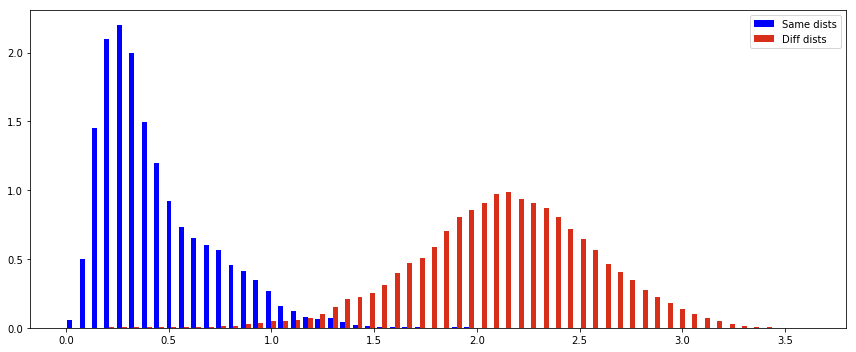
\includegraphics[width=15em,natwidth=856,natheight=352]{stats1/tl1.2_150_repartition.png} \\
		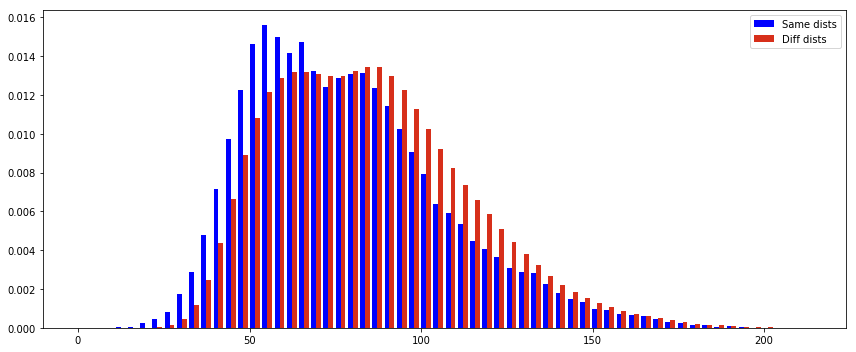
\includegraphics[width=15em,natwidth=856,natheight=352]{stats1/same_repartition.png}
		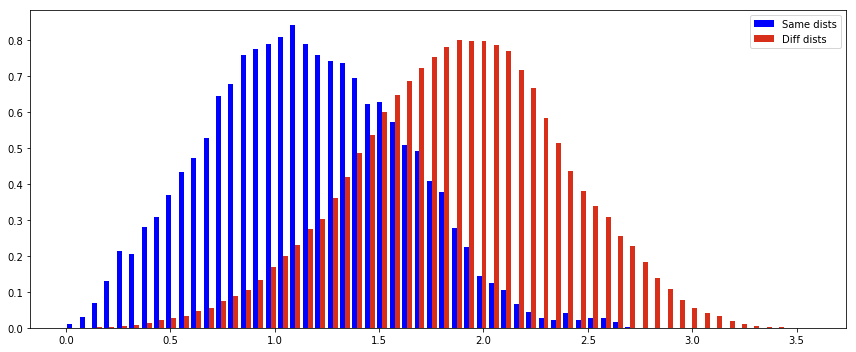
\includegraphics[width=15em,natwidth=856,natheight=352]{stats1/tl1_23in_repartition.png}
	\end{center}
\end{frame}

\section{Classification rapide avec K plus proches voisins}

\begin{frame}{Problème des k plus proches en dimension quelconque}
		\begin{center}
			\tikzimg{k_nearest_ne}
		\end{center}
		
		\begin{itemize}
			\item Nombre de dimensions : $d\in\mathbb{N}*$ ($d\in\{1,2,32\}$) (??)
			\item Nombre de points : $n\in\mathbb{N}*$ ($n\in\{10,10^2,10^3,10^4\}$) (??)
			\item Nombre de voisins : $k\in\mathbb{N}*$  ($k\in\{1,2,3,5\}$) (??)
		\end{itemize}
	\end{frame}

\begin{frame}{Approche par force brute}
	\begin{block}{Idée}
		Parcourir tous les points en maintenant les plus proches avec un tas.
	\end{block}

	Somes stats ???
	
	\begin{block}{Complexité}
			$O(n)$ si $k=1$, $O(n\ln(k))$ si $k>1$
	\end{block}
\end{frame}

\begin{frame}{K-d tree ($k=1$ uniquement)}
	%\begin{block}{Idée}
	%	Séparer récursivement les points par un hyperplan, puis rechercher avec un branch-and-bound.
	%\end{block}
	
	\begin{center}
		\tikzimg[width=\textwidth]{kdtree}
	\end{center}
	
	
	%\begin{block}{Complexité}
	%	Probabiliste. De $O(\ln(m))$ à $O(n)$
	%\end{block}
\end{frame}

\begin{frame}{Autres méthodes}
	TODO : stats de vitesse ET de \% de réussite pour toutes les méthodes
\end{frame}

\begin{frame}{Résultats (lesquels ?)}
	$$
	k=1, d=2
	$$
	\begin{center}\begin{tabular}{ |m{8em}|m{3.5em}|m{3.5em}| }
		\hline
		Algo & $n=10^2$ & $n=10^3$\\
		\hline
		\textbf{Force brute} & $100\%$ & $100\%$ \\
		\hline
	\end{tabular}\end{center}
\end{frame}

\section{Conclusion}

\begin{frame}[standout]
	Fin
\end{frame}

\end{document}
